\documentclass[]{article}
\usepackage{lmodern}
\usepackage{amssymb,amsmath}
\usepackage{ifxetex,ifluatex}
\usepackage{fixltx2e} % provides \textsubscript
\ifnum 0\ifxetex 1\fi\ifluatex 1\fi=0 % if pdftex
  \usepackage[T1]{fontenc}
  \usepackage[utf8]{inputenc}
\else % if luatex or xelatex
  \ifxetex
    \usepackage{mathspec}
  \else
    \usepackage{fontspec}
  \fi
  \defaultfontfeatures{Ligatures=TeX,Scale=MatchLowercase}
\fi
% use upquote if available, for straight quotes in verbatim environments
\IfFileExists{upquote.sty}{\usepackage{upquote}}{}
% use microtype if available
\IfFileExists{microtype.sty}{%
\usepackage{microtype}
\UseMicrotypeSet[protrusion]{basicmath} % disable protrusion for tt fonts
}{}
\usepackage[margin=1in]{geometry}
\usepackage{hyperref}
\hypersetup{unicode=true,
            pdftitle={Standardization \& Balancing: Utilization Table data-table and Shiny App description},
            pdfauthor={Cristina Muschitiello~Food and Agriculture Organization of the United Nations},
            pdfkeywords={Utilization Table, Rank, Inverse Ranking, Utilization, supply Commodity
Tree, FBS, CPC, shares, extraction Rates, conversion factors},
            pdfborder={0 0 0},
            breaklinks=true}
\urlstyle{same}  % don't use monospace font for urls
\usepackage{graphicx,grffile}
\makeatletter
\def\maxwidth{\ifdim\Gin@nat@width>\linewidth\linewidth\else\Gin@nat@width\fi}
\def\maxheight{\ifdim\Gin@nat@height>\textheight\textheight\else\Gin@nat@height\fi}
\makeatother
% Scale images if necessary, so that they will not overflow the page
% margins by default, and it is still possible to overwrite the defaults
% using explicit options in \includegraphics[width, height, ...]{}
\setkeys{Gin}{width=\maxwidth,height=\maxheight,keepaspectratio}
\IfFileExists{parskip.sty}{%
\usepackage{parskip}
}{% else
\setlength{\parindent}{0pt}
\setlength{\parskip}{6pt plus 2pt minus 1pt}
}
\setlength{\emergencystretch}{3em}  % prevent overfull lines
\providecommand{\tightlist}{%
  \setlength{\itemsep}{0pt}\setlength{\parskip}{0pt}}
\setcounter{secnumdepth}{5}
% Redefines (sub)paragraphs to behave more like sections
\ifx\paragraph\undefined\else
\let\oldparagraph\paragraph
\renewcommand{\paragraph}[1]{\oldparagraph{#1}\mbox{}}
\fi
\ifx\subparagraph\undefined\else
\let\oldsubparagraph\subparagraph
\renewcommand{\subparagraph}[1]{\oldsubparagraph{#1}\mbox{}}
\fi

%%% Use protect on footnotes to avoid problems with footnotes in titles
\let\rmarkdownfootnote\footnote%
\def\footnote{\protect\rmarkdownfootnote}

%%% Change title format to be more compact
\usepackage{titling}

% Create subtitle command for use in maketitle
\newcommand{\subtitle}[1]{
  \posttitle{
    \begin{center}\large#1\end{center}
    }
}

\setlength{\droptitle}{-2em}
  \title{Standardization \& Balancing: \texttt{Utilization\ Table}\\
data-table and Shiny App description}
  \pretitle{\vspace{\droptitle}\centering\huge}
  \posttitle{\par}
  \author{Cristina Muschitiello~Food and Agriculture Organization of the United
Nations}
  \preauthor{\centering\large\emph}
  \postauthor{\par}
  \predate{\centering\large\emph}
  \postdate{\par}
  \date{21 June 2018}

\usepackage{lscape}
\usepackage{booktabs}
\usepackage{longtable}
\usepackage{array}
\usepackage{multirow}
\usepackage[table]{xcolor}
\usepackage{wrapfig}
\usepackage{float}
\usepackage{colortbl}
\usepackage{pdflscape}
\usepackage{tabu}
\usepackage{threeparttable}
\usepackage{threeparttablex}
\usepackage[normalem]{ulem}
\usepackage{makecell}

\usepackage{draftwatermark}
\usepackage{makeidx}
\makeindex
\usepackage{float}
\floatplacement{figure}{H}
\usepackage{amsmath}
\usepackage{amssymb}
\usepackage{amsthm}
\usepackage{mathtools}
\usepackage{caption}

\begin{document}
\maketitle
\begin{abstract}
This vignette provides a description of the \texttt{Utilization\ Table}
data table: The data table is used in the Standardization and balancing
Process and is built from Old Sua Data. Also a shiny App for exploring
Old Sua, and see how the table has been built, is described
\end{abstract}

{
\setcounter{tocdepth}{4}
\tableofcontents
}
\href{https://unfao-my.sharepoint.com/:u:/g/personal/cristina_muschitiello_fao_org/EY8G-QNTrfBBjtm-4duSCY8BT8Ebp7ODhyMqgVE4Phz77A?e=vJzHPg}{\emph{Download
UtilizationTableApp from Share Point (select the zip file and download
it)}}

\newpage

\listoftables

\listoffigures

\subsection*{Disclaimer}\label{disclaimer}
\addcontentsline{toc}{subsection}{Disclaimer}

This Working Paper should not be reported as representing the official
view of the FAO. The views expressed in this Working Paper are those of
the author and do not necessarily represent those of the FAO or FAO
policy. Working Papers describe research in progress by the authors and
are published to elicit comments and to further discussion.

This paper is dynamically generated on \today{} and is subject to
changes and updates.

\newpage

\section{Introduction}\label{introduction}

This document is part of a series of documents concerning Food Balance
Sheets and their computation. Other documents describe the steps for the
computation of Food Balance Sheets and, in particular, the
Standardization and Balancing process. The Standardization is the
conversion of the variables of any child commodity in the
primary-equivalent commodity. One of the main steps of the
standardization is the, so called, \emph{Sua Filling}. In this step, an
automatic check is performed on the Supply-utilization accounts, for the
existence of figures for all the Variables that are required for the
specific commodity. The algorithm that performs this check, make use of
the history of that commodity. The history is given by time series of
SUAs for each country-commodity combination. This information is stored
in a table called \emph{Utilization Table}.

\section{The Utilization Table in The
SWS}\label{the-utilization-table-in-the-sws}

The Table is stored inside the Statistical Working System as a
\texttt{Data\ table} in the \texttt{SUA/FBS} domain (figures
\ref{fig:f1} and \ref{fig:f2}).

\begin{figure}[H]

{\centering 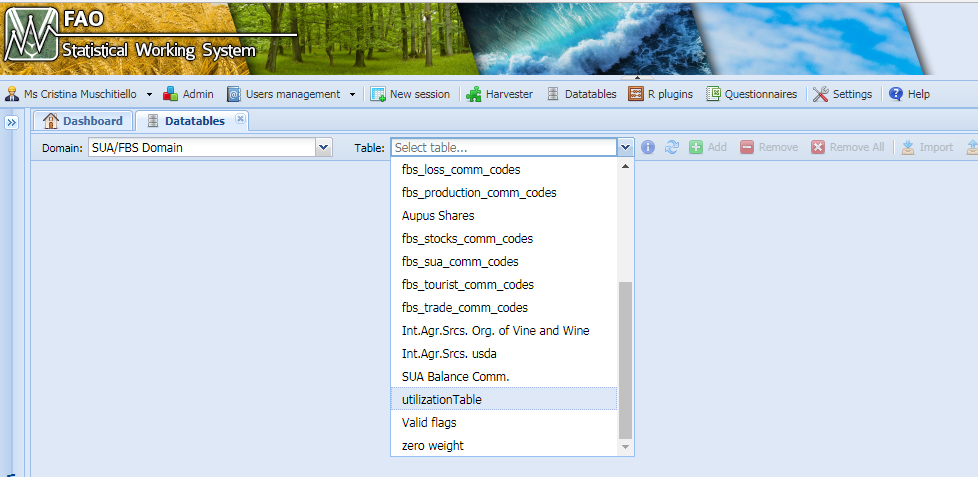
\includegraphics[width=0.9\linewidth]{images/UtilizationTable/01_domainSelection} 

}

\caption{\label{fig:f1}Selection of domain and Data - Table in the Statistical Working System}\label{fig:f1}
\end{figure}

Information is given in codes:

\begin{itemize}
\tightlist
\item
  \texttt{geographicAreaM49} is the M49 country code
\item
  \texttt{measuredElementSuaFbs} is the Element name
\item
  \texttt{measuredItemSuaFbs} is the \emph{CPC} item code
\item
  \texttt{rank} is the rank
\item
  \texttt{rankInv} is the Inverse Rank
\end{itemize}

The table is not very user friendly, but it can be filtered for a
clearer use.

\begin{figure}[H]

{\centering 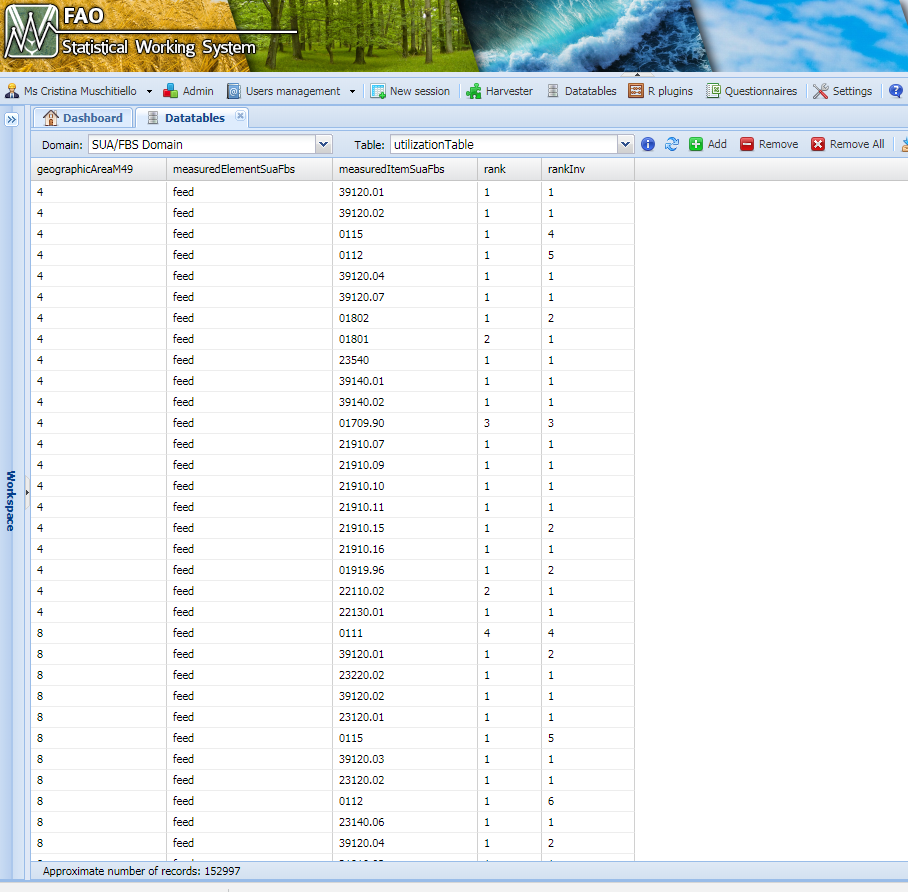
\includegraphics[width=0.9\linewidth]{images/UtilizationTable/02_UTilizationTable} 

}

\caption{\label{fig:f2}Utilization Table in the FAO Statistical Working System}\label{fig:f2}
\end{figure}

For example, figures \ref{fig:f3} and \ref{fig:f4} represent the
Utilization Table filtered for Flour of wheat in China, Main.

\begin{figure}[H]

{\centering 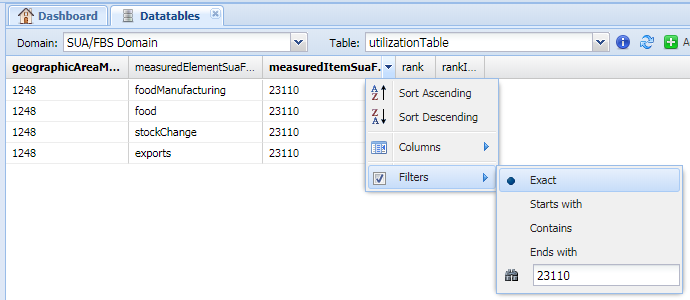
\includegraphics[width=0.9\linewidth]{images/UtilizationTable/03_filter1} 

}

\caption{\label{fig:f3}filtering Utilization Table}\label{fig:f3}
\end{figure}

\begin{figure}[H]

{\centering 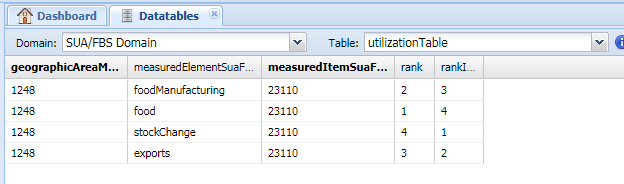
\includegraphics[width=0.9\linewidth]{images/UtilizationTable/04_filter2} 

}

\caption{\label{fig:f4}Utilization Table  filtered for China, Main - Flour of Wheat}\label{fig:f4}
\end{figure}

\section{Content}\label{content}

The \emph{Utilization table} is a country-commodity specified table
containing, for each country-commodity combination:

\begin{enumerate}
\def\labelenumi{\arabic{enumi}.}
\tightlist
\item
  The list of the Variables
\item
  A rank for each variable, identifying the \emph{rank of the mean value
  over the period 2000-2013}
\item
  The rank Inverse
\end{enumerate}

\subsection{The list of variables}\label{the-list-of-variables}

The Variables listed are all the variables that have been historically
active for that Country-commodity combination. In other words, if the
commodity has never been traded, no Import or Export will appear, if it
has never been used for feed, no feed will appear and so on.

This is the first information included in the table. Indeed, the
Standardization and Balancing would not have any source telling which
variables are expected to be active for a specific country-commodity
combination, if this table didn't exist.

\subsection{The Rank}\label{the-rank}

The Rank appearing in the table is built using the mean value of that
variable in the time range 2000-2013. This time range has been used for
the majority of validation procedure used for the new methodology. 2013
is the last year in which FBSs were produced using the old methodology,
therefore it is used as last year.

\subsection{The Inverse Rank}\label{the-inverse-rank}

The Inverse Rank is added in the table for computation reasons. An
algorithm has been developed indeed, which uses Ranks and inverse Ranks
for distributing The Imbalance in the Supply-Utilization accounts during
the Standardization procedure.

\section{A Shiny App to explore How the Utilization Table is
built}\label{a-shiny-app-to-explore-how-the-utilization-table-is-built}

The Utilization table is given as a Data Table. There is NOT a module or
plug-in for changing it, therefore a tool is needed for at least explore
the data it is built on. A shiny tool has been developed for this
purpose. The main aim of the App is that of knowing where the table is
from. Possible actions are:

\begin{itemize}
\tightlist
\item
  change directly the values in the Data-Table inside the SWS
\item
  Develop a new ad-hoc approach.
\end{itemize}

\subsection{Download the App}\label{download-the-app}

The App can be downloaded from FAO SharePoint:

\href{https://unfao-my.sharepoint.com/:u:/g/personal/cristina_muschitiello_fao_org/EY8G-QNTrfBBjtm-4duSCY8BT8Ebp7ODhyMqgVE4Phz77A?e=vJzHPg}{\emph{Download
UtilizationTableApp from Share Point (select the zip file and download
it)}}

Or it can be found in the ESS T-DRIVE at the following address:

\texttt{T:\textbackslash{}Team\_working\_folder\textbackslash{}A\textbackslash{}FBS-Modules\textbackslash{}Balancing-standardization}

\subsection{Open and run the App}\label{open-and-run-the-app}

\begin{itemize}
\tightlist
\item
  unzip the folder
\item
  run the .vbs file included (figure \ref{fig:f5})
\item
  wait for the Browser to open the page (figure \ref{fig:f6})
\end{itemize}

\begin{figure}[H]

{\centering 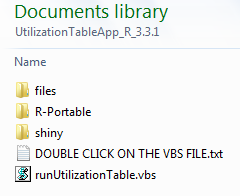
\includegraphics[width=0.6\linewidth]{images/UtilizationTable/05_folderApp} 

}

\caption{\label{fig:f5}Run Shiny App}\label{fig:f5}
\end{figure}

\subsection{Content}\label{content-1}

The App has two main pages:

\begin{enumerate}
\def\labelenumi{\arabic{enumi}.}
\tightlist
\item
  UTILIZATION TABLE
\item
  Exploring Old Sua
\end{enumerate}

In the first page the Utilization table can be explored (figure
\ref{fig:f6}). Is possible to scroll down the page or filter by one or
all the Variables.

\begin{figure}[H]

{\centering 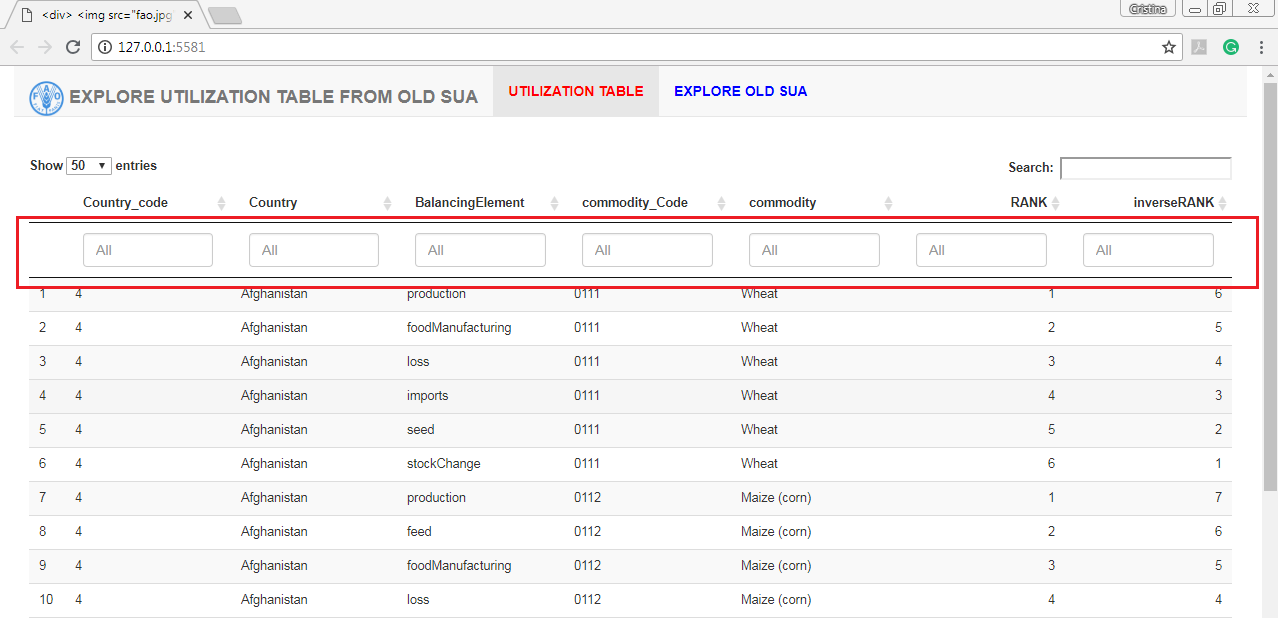
\includegraphics[width=1\linewidth]{images/UtilizationTable/06_Browser1} 

}

\caption{\label{fig:f6}Shiny App Main Page - Utilization Table Page}\label{fig:f6}
\end{figure}

The second page is for exploring the Data from which the table has been
built (figure \ref{fig:f7}).

\begin{figure}[H]

{\centering 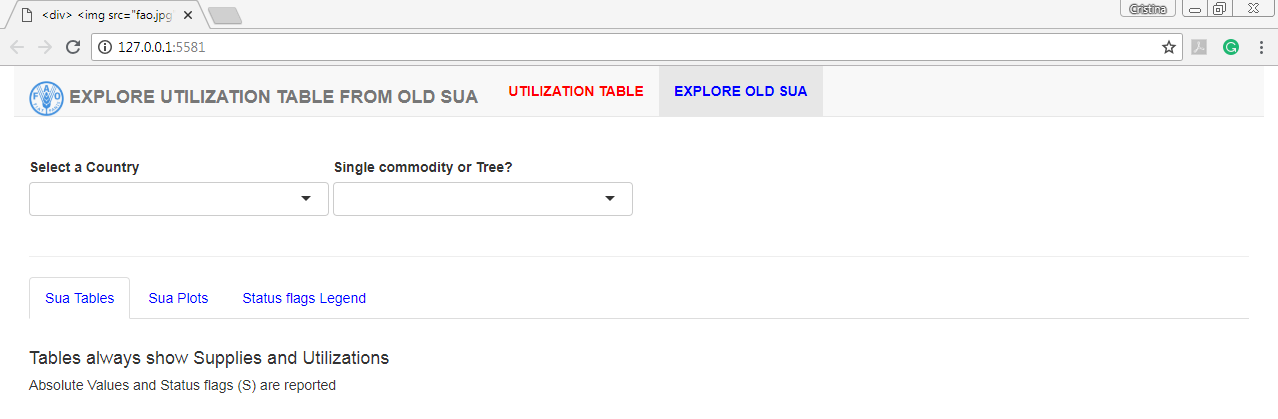
\includegraphics[width=1\linewidth]{images/UtilizationTable/07_Browser2_explore} 

}

\caption{\label{fig:f7}Shiny App 'Ranking old Sua' Page}\label{fig:f7}
\end{figure}

After having selected the country (figure \ref{fig:f8}) is possible to
visualize table and Plot of a single commodity or a commodity tree
(figures \ref{fig:f9} to \ref{fig:f11}). If the ``tree'' option is
selected, a new field appears for selecting the Primary (or proxy
primary) \footnote{notice that the Commodity Tree might be a bit changed
  since this App was created, therefore some difference might exist}.

\begin{figure}[H]

{\centering 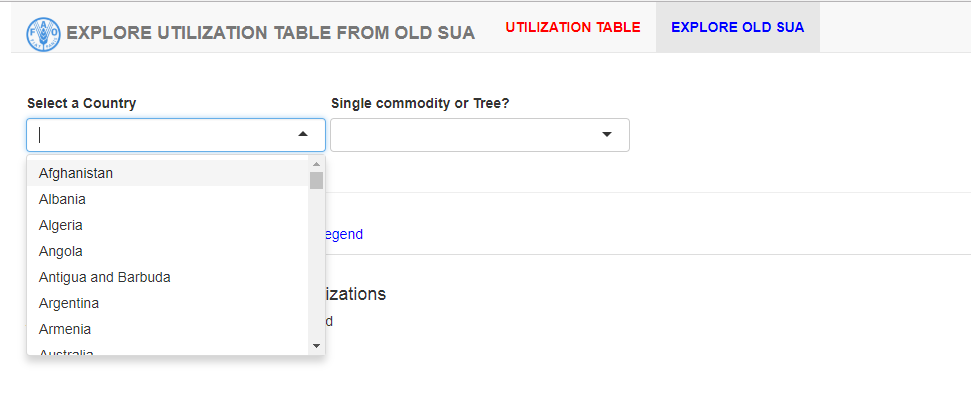
\includegraphics[width=1\linewidth]{images/UtilizationTable/08_selectCountry} 

}

\caption{\label{fig:f8}Shiny App - Select Country}\label{fig:f8}
\end{figure}

\begin{figure}[H]

{\centering 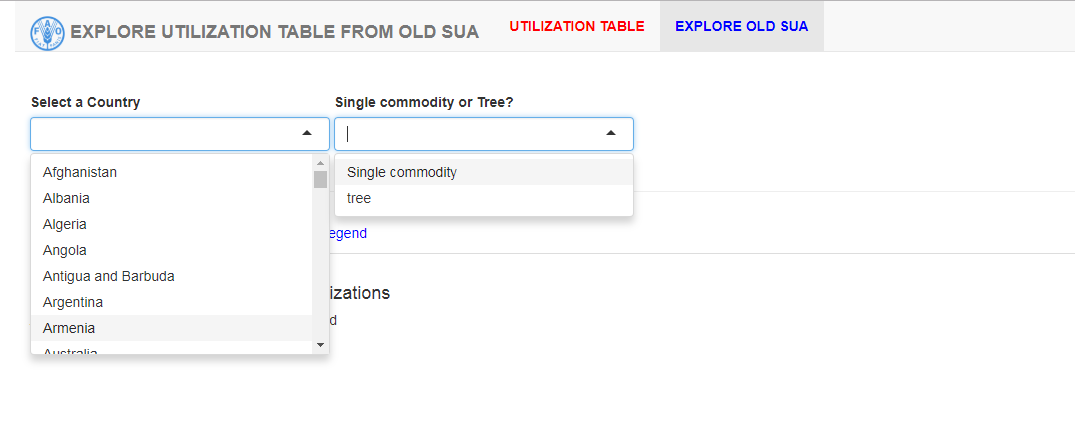
\includegraphics[width=1\linewidth]{images/UtilizationTable/09_selectCommodityTre} 

}

\caption{\label{fig:f9}Shiny App - Select Commodity or Tree}\label{fig:f9}
\end{figure}

\begin{figure}[H]

{\centering 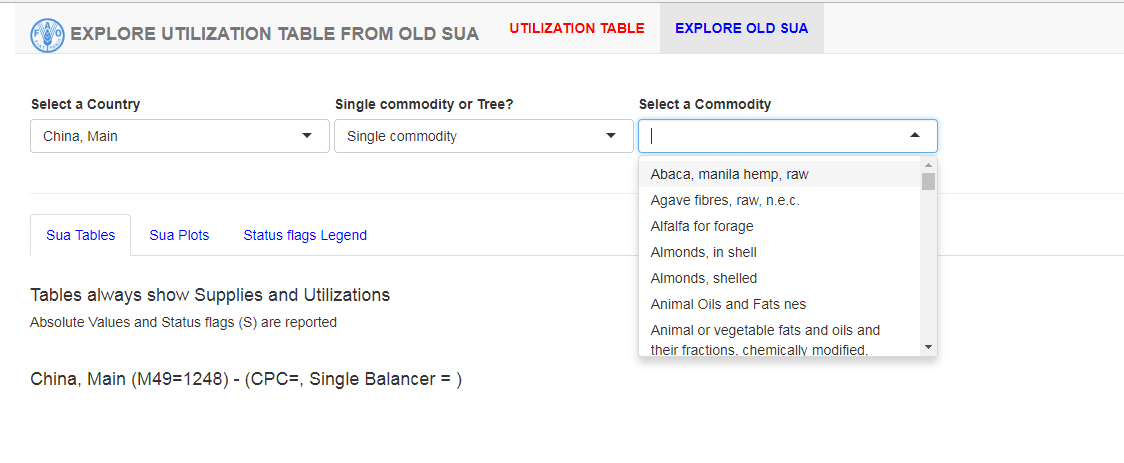
\includegraphics[width=1\linewidth]{images/UtilizationTable/10_selectComm} 

}

\caption{\label{fig:f10}Shiny App - Select Commodity}\label{fig:f10}
\end{figure}

\begin{figure}[H]

{\centering 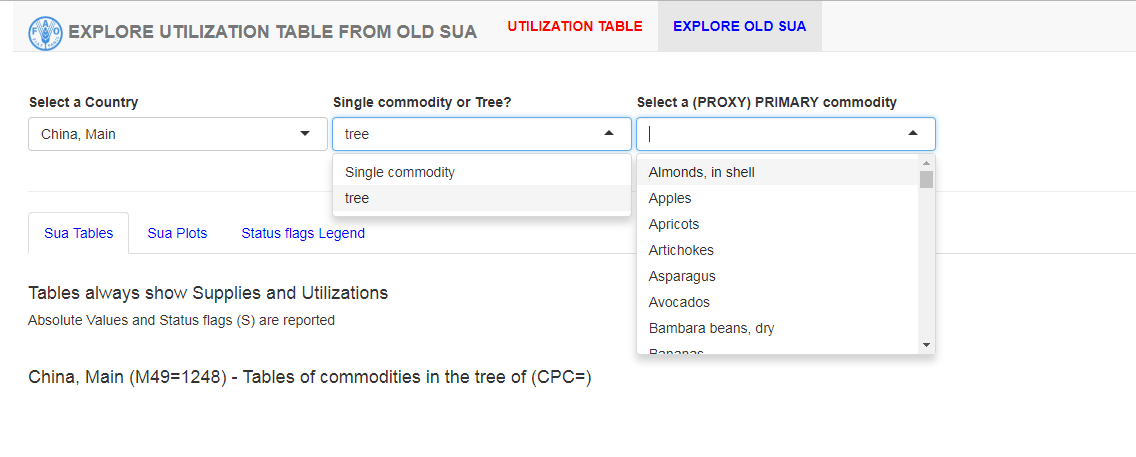
\includegraphics[width=1\linewidth]{images/UtilizationTable/11_selectPrimary} 

}

\caption{\label{fig:f11}Shiny App - Select (PROXY) PRIMARY commodity}\label{fig:f11}
\end{figure}

For each commodity or Commodity Tree selected there is a tab containing
tables (figure \ref{fig:f12}) and a second tab containing plots (figure
\ref{fig:f13}). In the table there are separate columns for Flags. The
legend of flags is reported in the \emph{Status flag legend} tab (figure
\ref{fig:f15}).

\begin{figure}[H]

{\centering 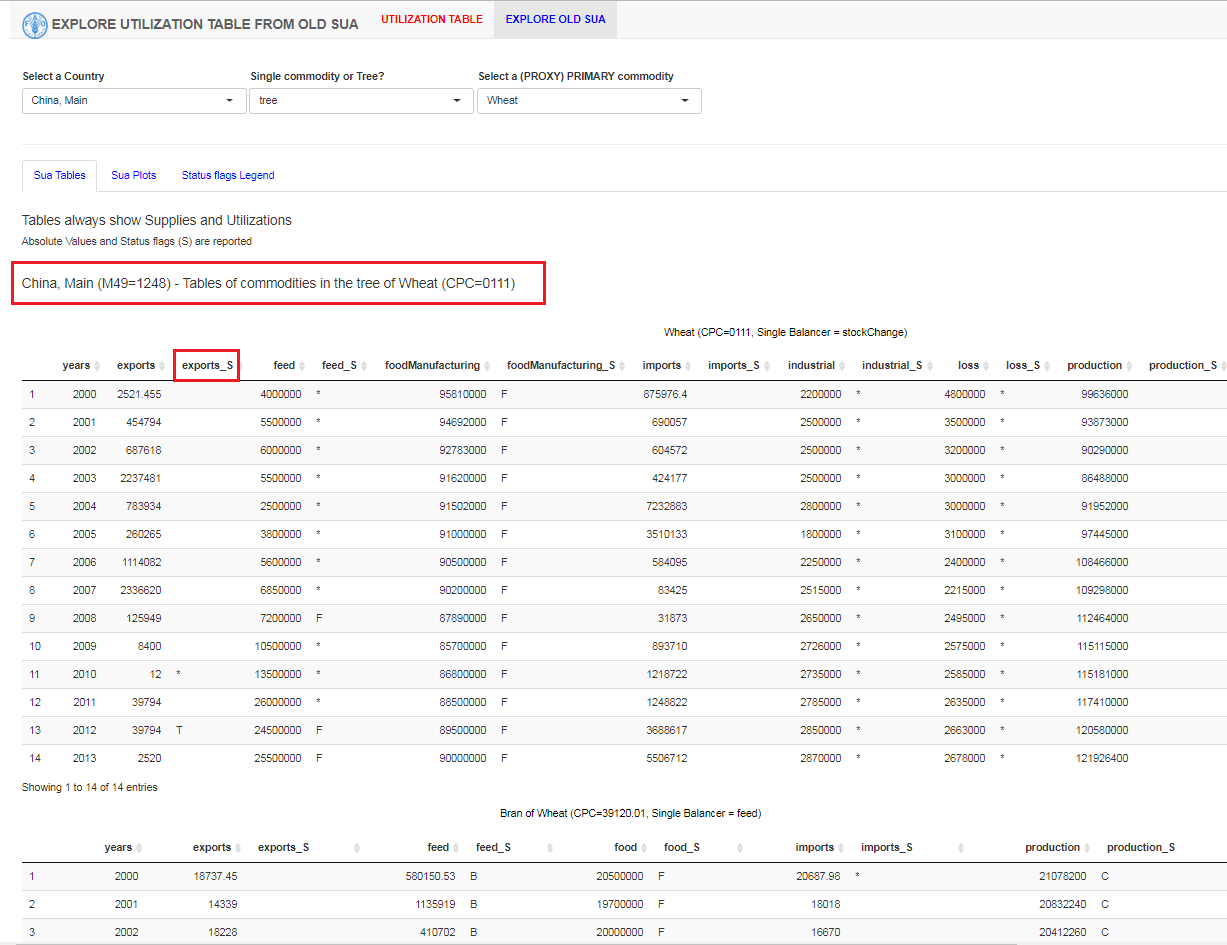
\includegraphics[width=1\linewidth]{images/UtilizationTable/12_treeTableVisual} 

}

\caption{\label{fig:f12}Shiny App - 'Sua Table' window}\label{fig:f12}
\end{figure}

Plots are interactive, i.e.~the Value is shown when the mouse pass on a
point. Also the Single Balancer reported\footnote{This is the variable
  used as Balancer in the Previous Approach}. Plots report both supply
and utilization. Is possible to show only supply or utilization (figure
\ref{fig:f14}).

\begin{figure}[H]

{\centering 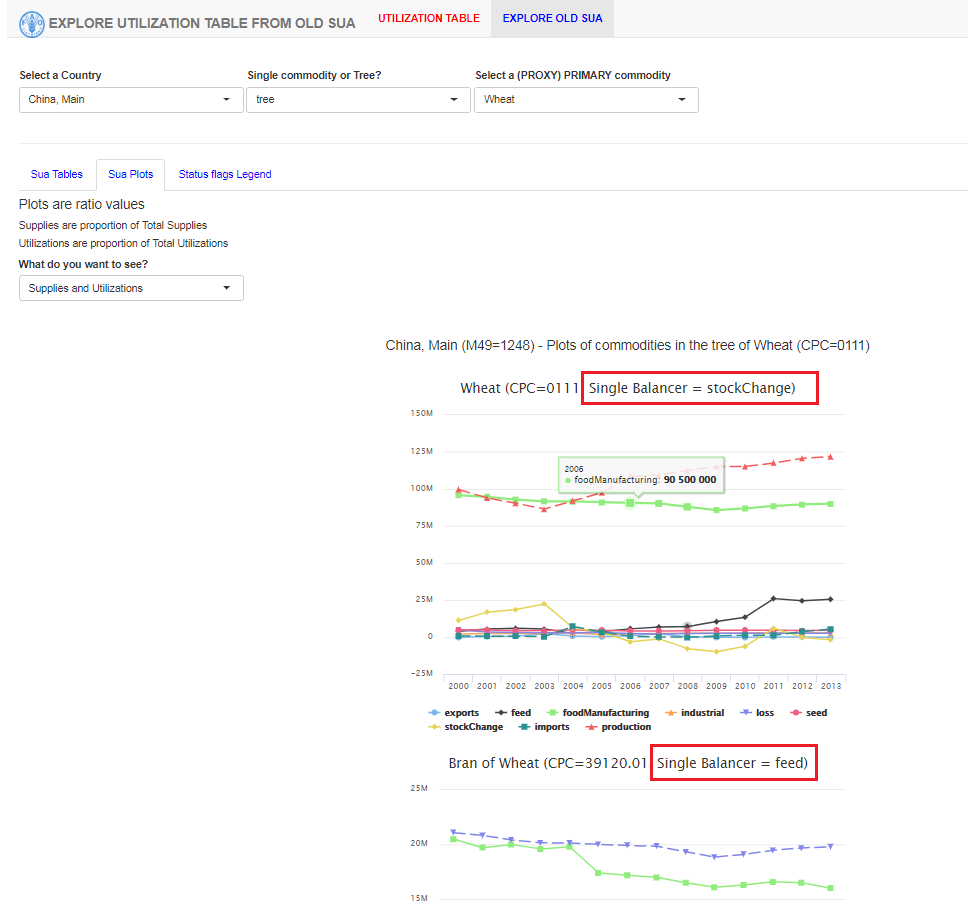
\includegraphics[width=1\linewidth]{images/UtilizationTable/13_treePlotVisual} 

}

\caption{\label{fig:f13}Shiny App - 'Sua Plots' window}\label{fig:f13}
\end{figure}

\begin{figure}[H]

{\centering 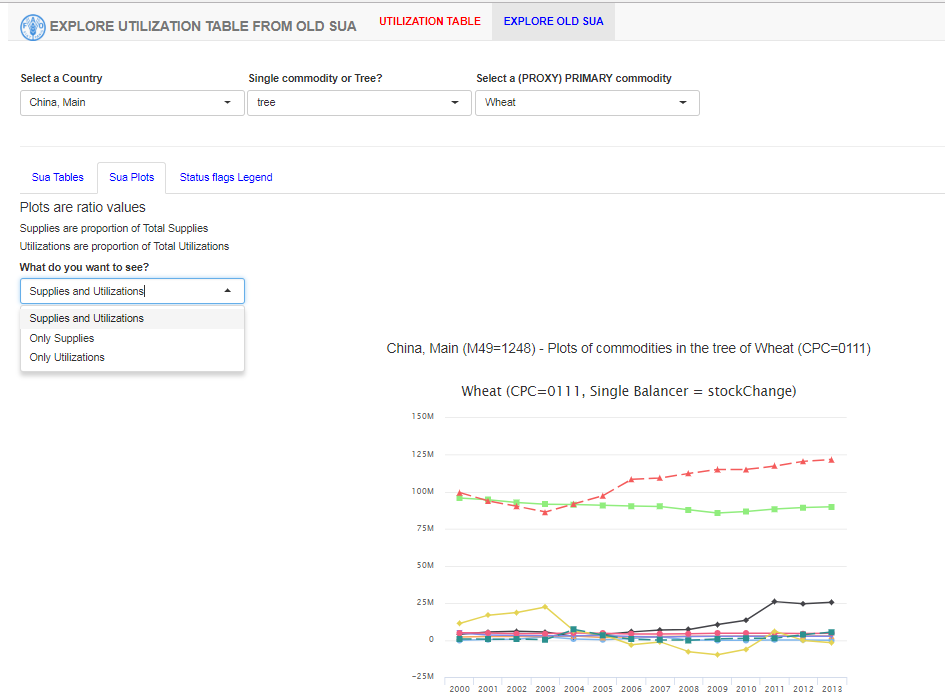
\includegraphics[width=1\linewidth]{images/UtilizationTable/14_selectsupUtil} 

}

\caption{\label{fig:f14}Shiny App - select visualization: Supply and/or utilization}\label{fig:f14}
\end{figure}

\begin{figure}[H]

{\centering 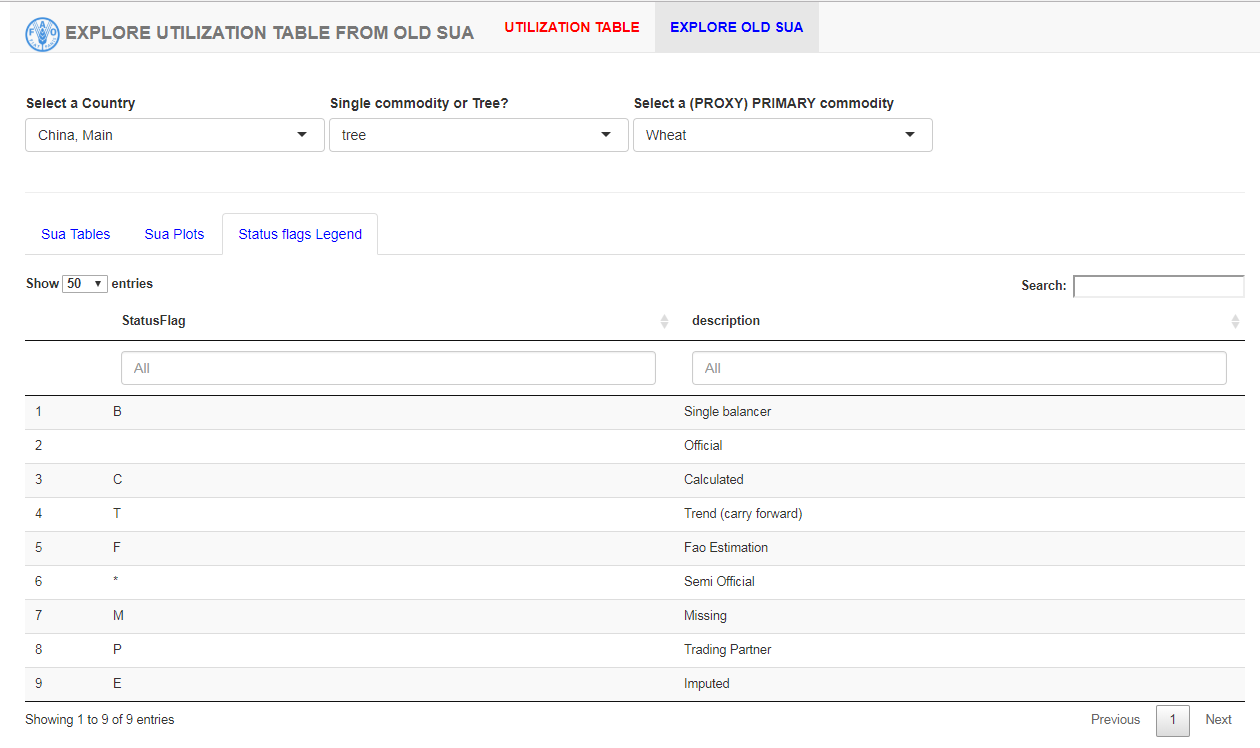
\includegraphics[width=1\linewidth]{images/UtilizationTable/15_Flags} 

}

\caption{\label{fig:f15}Shiny App - Flags}\label{fig:f15}
\end{figure}


\end{document}
